% !TeX spellcheck = en_US
\documentclass{article}

\usepackage{graphicx}

\usepackage[cp1250]{inputenc}
\usepackage[lastpage,user]{zref}
\usepackage[table,xcdraw]{xcolor}
\usepackage{pdfpages}
\usepackage{graphicx}
\usepackage[export]{adjustbox}
\usepackage{tabu}

\begin{document}

\vspace*{3ex}
\begin{flushright}
{\large 7 March 2015}
\end{flushright}

\begin{flushleft}
{\large Lukasz W�jcik\\

}
\end{flushleft}

\hskip3cm

\begin{center}

\Large {\bf
	Individual project
}

\Large {\bf
	Cellular automaton
}

\Large {\bf 
	Requirement specification 
}

\vskip2ex

\vspace{50pt}

\includegraphics[width=100mm]{images/mini.png} \\

\end{center}

\vskip20ex
\label{LastPage}
\begin{flushleft}
{\fontsize{10cm}{1em} {\bf Informations}\\
}
\end{flushleft}

\vskip2ex
\begin{flushleft}
{\huge Scheldue\\
}
\end{flushleft}
\begin{center}
\begin{table}[h]
\begin{tabular}{|l|l|}
\hline
\rowcolor[HTML]{BF6969} 
{\color[HTML]{000000} Date} & {\color[HTML]{000000} Stage} \\ \hline
2015-03-12                  & requirement specification    \\ \hline
2015-04-02                  & technical project            \\ \hline
2015-04-23                  & code of modules              \\ \hline
2015-04-30                  & version 0.98                 \\ \hline
2015-05-07                  & version 0.99                 \\ \hline
2015-05-14                  & version 1.0                  \\ \hline
2015-05-21                  & test report                  \\ \hline
2015-06-11                  & acceptation                  \\ \hline
\end{tabular}
\end{table}
\end{center}

\begin{flushleft}
{\huge Document metric\\
}
\end{flushleft}

\begin{table}[h]
\begin{tabular}{|
>{\columncolor[HTML]{BF6969}}l |l|l|l|l|l|}
\hline
\multicolumn{6}{|l|}{\cellcolor[HTML]{BF6969}\textbf{Document metric}}                                                                                                               \\ \hline
\textbf{Project:}       & \multicolumn{2}{l|}{Cellular automaton}          & \cellcolor[HTML]{BF6969}\textbf{Company:} & \multicolumn{2}{l|}{WUT}                                    \\ \hline
\textbf{Name:}          & \multicolumn{5}{l|}{Cellular Automata requirement specification}                                                                                           \\ \hline
\textbf{Topics:}        & \multicolumn{5}{l|}{Features of Cellular Automata program}                                                                                                 \\ \hline
\textbf{Author:}        & \multicolumn{5}{l|}{Lukasz W�jcik}                                                                                                                         \\ \hline
\textbf{File:}          & \multicolumn{5}{l|}{cellular\_automata\_requirement\_specification}                                                                                        \\ \hline
\textbf{Version no:}    & 0.1 & \cellcolor[HTML]{BF6969}\textbf{Status:} & Designing                                 & \cellcolor[HTML]{BF6969}\textbf{Opening date:} & 2015-02-26 \\ \hline
\textbf{Summary:}       & \multicolumn{5}{l|}{Providing business analysis and requirement specification.}                                                                            \\ \hline
\textbf{Authorized by:} & \multicolumn{2}{l|}{Wladyslaw Homenda}           & \multicolumn{2}{l|}{\cellcolor[HTML]{BF6969}\textbf{Last modification date:}}              & 2015-03-11 \\ \hline
\end{tabular}
\end{table}
\begin{flushleft}
{\huge Changes\\
}
\end{flushleft}
\begin{table}[h]
\begin{tabular}{|l|l|l|l|}
\hline
\rowcolor[HTML]{BF6969} 
\multicolumn{4}{|l|}{\cellcolor[HTML]{BF6969}\textbf{History of changes}}     \\ \hline
\rowcolor[HTML]{E3DBDB} 
Version & Date       & Who           & Description                            \\ \hline
0.1     & 2015-03-11 & Lukasz W�jcik & Creation of requirements specification \\ \hline
\end{tabular}
\end{table}
\newpage
\tableofcontents
\vskip5ex
\begin{flushleft}
{\huge Short summary of documentation\\
}
\end{flushleft}
\Large\hspace{15pt}This document is a requirement specification of Cellular automation program.
\newpage
\section{Production model} \par
\Large\hspace{15pt}STH
\newpage
\section{Concepts vocabulary}
\hspace{15pt}\Large {\bf Cellular automaton } - consists of a regular grid of cells, each in one of a finite number of states (in our case 0 and 1). The grid is two dimensional. For each cell, a set of cells called its neighborhood is defined relatively to the specified cell. An initial state is selected by assigning a state for each cell. A new generation is created, according to some fixed rule that determines the new state of each cell in terms of the current state of the cell and the states of the cells in its neighborhood. Typically, the rule for updating the state of cells is the same for each cell and does not change over time, and is applied to the whole grid simultaneously. \\

\hspace{15pt}\Large {\bf Grid } - in this project, grid is a 2D matrix with finite numbers of rows and columns. \\

\Large {\hspace{15pt}\bf Cell} - the smallest part of grid which has its state (0 or 1, black or white) and neighborhood. \\
\newpage
\Large {\bf Neighborhood} - state of cell in next iteration depends on rule and its neighbors. In this project three types neighborhood are considered:
	\begin{itemize}
	
	\item	
		4 points neighborhood \hspace{50pt} 
			 
\includegraphics[width=30mm]{images/4_neigh.png} \\

	\item	
		8 points neighborhood \hspace{50pt}
			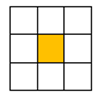
\includegraphics[width=30mm]{images/8_neigh.png} \\

	\item	
		24 points neighborhood \hspace{50pt}
			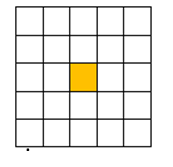
\includegraphics[width=30mm]{images/24_neigh.png} \\				
	\end{itemize}
\newpage
\section{User stories}
	
	\hspace*{-2.1cm}
		\begin{tabular}{| l | p{15cm}|}
		
			\hline
		  	Nr. & User story \\
			\hline
			
			1 & 
		{\bf As a beginner user}, 
					I want have easy access to help or tutorial.
			\\ \hline
	
			2 & 
				{\bf As a user}, 
						I want to be able to change size of a grid.
			\\ \hline
	
			3 & 
			{\bf As a user}, 
						I want to be able to set initial state for each cell in the grid drawing  with my mouse and save it.
			\\ \hline
			
			4 & 
				{\bf As a user}, 
						I want to be able to create and save my own rules.
			\\ \hline
	
			5 & {\bf As a user},I want to be able to create and save my own cells states.\\ \hline
			
			6 & {\bf As a user},I want to have an easy way to explore files with rules and cells states stored on my disk.\\ \hline
			
			7 & {\bf As a user},I want to make computations step by step or by N steps where N is provided by me.\\ \hline	
	
			8 & 
			{\bf As a user who has been using this program before}, 
						I want to be able to load previously saved states for cells in a grid.
			\\ \hline
			9 & {\bf As a user who has been using this program before}, 
					I want to be able to load previously saved rules.\\ \hline
					
			10 & {\bf As a user who want to exit the program},I want to be able to exit the program in any time. I also want to be informed about ongoing computations or changes which has not been saved\\ \hline		
	
	
		  \hline
		\end{tabular}
\newpage
\section{Functional Requirements}

	\hspace*{-2.1cm}
		\begin{tabular}{| l | p{15cm}|}
		
			\hline
		  	Nr. & Functional requirement \\
			\hline
			
			1 & Clicking on "Rules" folder in a left section of the main window of a program should expand a tree with a system of folders and files with previously saved rules.Double click on a file with a rule will load that rule into the program. Next click on a "Rules folder should collapse a file tree. 
			\\ \hline
			2 & Clicking on the "Cells states" folder in left section of main window of program should expand a tree with system of folders and files with previously saved cells states. Double click on file with cells state will load that state into the program. Next click on "Cells states" should collapse a file tree.
			\\ \hline
			3 & Scrolling with mouse scroll or pinching on touch pad should zoom in or zoom out the grid.
						\\ \hline
			4 & Clicking on a cell in the grid should change its state to opposite one (since we're dealing with binary states).
						\\ \hline
			5 & Dragging mouse over the grid with left button pressed should change state of cell over which the cursor was hovering to the opposite one.\\\hline
			6 & Clicking on "Edit grid" button will make a popup window appear. In the popup we will be able to set number of rows and number of columns of the grid. \\\hline
			7 & Clicking on "Save cells state" button will save current state of cells in grid to a file. User will be able to specify folder location and name of the file.\\\hline
			8 & Clicking "Edit rule" button will open popup window with tools to edit rule which is currently in use.
			 \\\hline
			9 & Clicking on "Save rule" button will save a current rule to a file. User will be able to specify a folder location and the name of the file.\\\hline 			

		  \hline
		\end{tabular}
		
		\newpage
		\hspace*{-2.1cm}
				\begin{tabular}{| l | p{15cm}|}
				
				\hline
				Nr. & Functional requirement \\	
					\hline
					
				10 & Clicking on "Files" button in menu bar on top of the program window will open a list of functions such as: create new rule,create new grid cells state. In rule creator, user will be able to choose neighborhood type (4,8 or 24 neighbors) and manually add principles determining state of each cell.\\\hline
				11 & Clicking on "Edit" button in top menu bar will open a list of functions which will provide tools to edit rules and cells states which are not currently in use.\\\hline
				12 & Clicking on "Settings" button in top menu bar will provide tools to change source of folders with rules and cells states. \\\hline
				13 & Clicking on "Help" button in top menu bar will show a list of functions such as: problems, tutorial, contact. "Problems" function will provide answers to most common problems (if such would exist)."Tutorial" function will be able to show to user how to use "Cellular automata" program step by step. Contact function will provide a way to contact with person responsible by functionality of this software. \\\hline
				14 & Clicking on "One step" button will execute computation of the next generation. If rule or initial state of cells will not be set, user will be prompted to do so.  \\\hline
				15 & Clicking on "N steps" button will execute computation of  next generation N times. If rule, initial state of cells or number of steps will not be set, user will be prompted to do so. \\\hline
				16 & User will be able to minimize,maximize or change the size of a program window. User will also be able to exit program in any time but he will be alarmed about any ongoing computations or not saved changes. \\\hline 			
		
				  \hline
				\end{tabular}
		\newpage
\section{Non Functional Requirements}

\hspace{15pt}\Large A user interface should be as clean and user friendly as it's only possible. Intuitive addition of rule sets. Software should be snappy, make use of new hardware (like multi-core processors) but also compatible with older devices. Computations should not block or slow down GUI. In case of some error (computer restart, system crash, etc.) user's work should be stored in a backup file which should be updated during software runtime.
\newpage
\section{GUI prototype}
\begin{figure}[h!]
		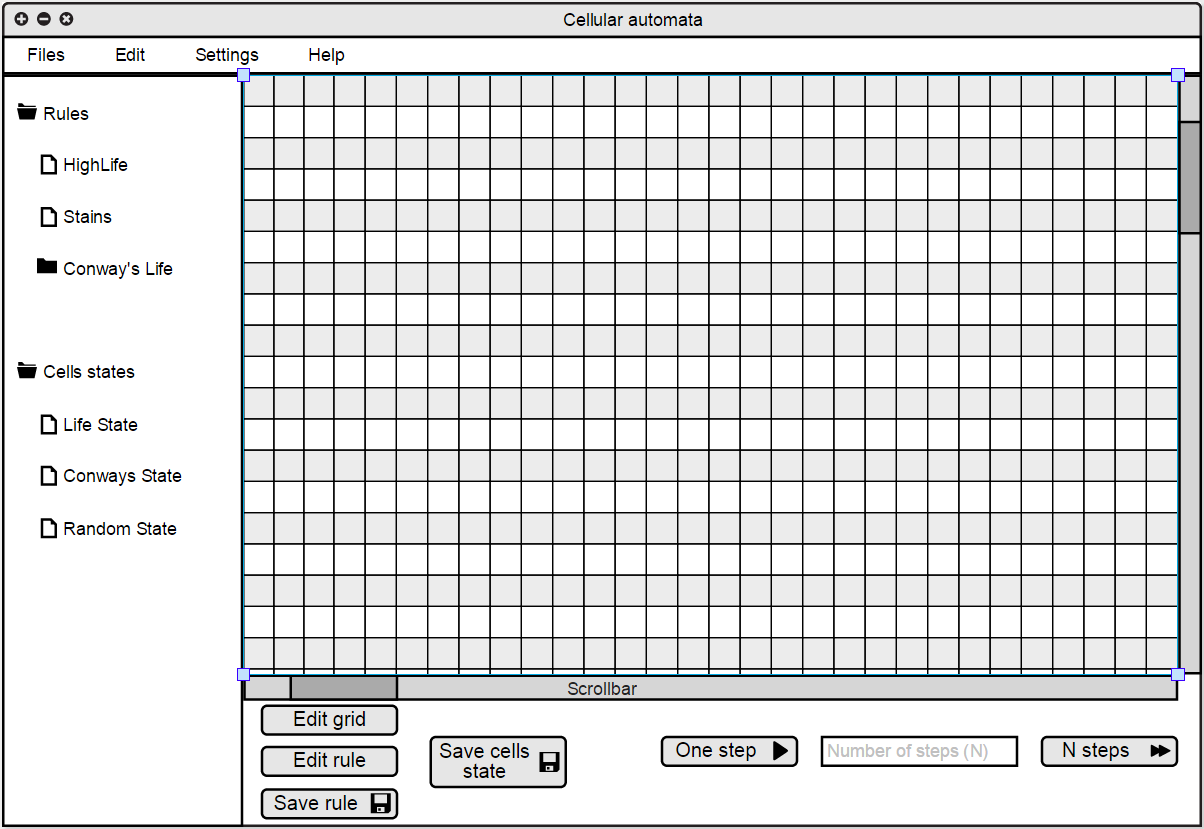
\includegraphics[page=1,width=1.5\textwidth, center]{images/gui_prototype}
\end{figure}

\hspace{15pt}\Large \\ User interface should be kept as simple and as clean as its possible. GUI prototype shown above consist of 4 components. Top menu bar has buttons forwarding to functions for modifying rules and cell states. It also contain application settings and help with tutorial. On the left there are two file trees with default and previously made rules and cells states. On the bottom there is a set of buttons for rules and cells states currently in use and buttons for starting computing of new generations.

\hspace{15pt}  User should have possibility to resize all components except menu bar.

	

\section{Evaluation of solution}
	\begin{itemize}
	
	\item	
		Correctness of solution
	\item	
		Meeting the requirements
	\item	
		Clarity \\					
	\end{itemize}

\section{Risk analysis}
\hspace{15pt}\Large One of the risk is not sticking to schedule on one of more stages of software development. Not meeting basic requirements stated on the begging might also be a big problem. Errors made on early stage of development can be very troublesome, since correcting it will most likely involve more work than it would right after creation of such error. Another problem which may occur is compatibility with different software environments (Windows,Linux).
\end{document}
